\chapter{Instalacja i wdrożenie}
\thispagestyle{chapterBeginStyle}

    W tym rozdziale opisane zostały wymagania i kolejne kroki potrzebne do uruchomienia aplikacji
oraz podstawowe operacje możliwe do wykonania w jej zakresie.



\section{Środowisko}
    Aplikacja opisana w tej pracy jest aplikacją mobilną. Do jej uruchomienia potrzebne jest
urządzenie mobilne z systemem Android. Działanie aplikacji zostało przetestowane na telefonie
z tym systemem w wersji 8.0 i zaleca się jej uruchomienie na tej wersji systemu.



\section{Instalacja}
    Proces instalacji rozpoczyna się od przeniesienia załączonego pliku \texttt{nogram.apk} na urządzenie.
Kroki opisane poniżej opisują przykładowy proces instalacji i mogą różnić się w zależności od wersji
systemu lub nakładki nałożonej na system.
\begin{enumerate}
    \item Znaleźć w pamięci urządzenia przeniesiony plik instalacyjny.
    \item Dotknąć ikony pliku, by rozpocząć proces instalacji.
    \item Na ekranie pojawi się komunikat z zapytaniem o chęć instalacji.
    \item Nacisnąć przycisk \textit{Instaluj}.
    \item Rozpocznie się proces instalacji aplikacji.
    \item W trakcie instalacji może pojawić się komunikat o zablokowaniu instalacji przez Play Protect,
z wyjaśnieniem, że aplikacja pochodzi od nieznanego dewelopera. Wynika to z braku zatwierdzenia
aplikacji w usługach firmy Google i instalacja nie stanowi zagrożenia dla urządzenia. Kontynuacja
instalacji jest możliwa po kliknięciu przycisku \textit{Zainstaluj mimo to}.
    \item System dokończy instalację aplikacji.
\end{enumerate}
    Uruchomienie aplikacji jest możliwe przez znalezienie jej ikony na liście aplikacji lub kliknięcie
przycisku \textit{Otwórz} na ekranie końcowym aplikacji.



\section{Obsługa}
    Po uruchomieniu aplikacji wyświetlony zostanie ekran główny, czyli ekran wyboru paczki łamigłówek.
Kolejne interakcje można prowadzić nawigując po systemie, zgodnie z diagramem przedstawionym w
rozdziale trzecim (\ref{diagAktywnosci}). Podstawowe operacje możliwe do wykonania w aplikacji
zostały opisane poniżej.


\subsection{Nawigacja do łamigłówki}
    Będąc w ekranie wyboru paczki łamigłówek, należy wybrać jedną z paczek poprzez kliknięcie jej
karty. Na ekranie wyświetli się lista łamigłówek. Kliknięcie karty jednej z nich otworzy planszę
do rozwiązania.

    Karta łamigłówki odzwierciedla jej stan. Na domyślnym, szarym tle, zaprezentowane są łamigłówki,
których nie udało się rozwiązać do tej pory. Srebrne tło oznacza łamigłówkę, która została rozwiązana,
ale przynajmniej raz użytkownik popełnił zbyt wiele błędów i musiał zacząć od nowa. Łamigłówki
ze złotym tłem to takie, które udało się rozwiązać za pierwszym razem. Stan łamigłówki, wraz z
układem pól na planszy, jest zapisany przy wyjściu. Co więcej, o stanie łamigłówki świadczy ikona
wyświetlana na jej karcie, która odróżnia łamigłówki rozpoczęte od nierozpoczętych.

    Na karcie paczki łamigłówek pokazany jest postęp w jej rozwiązaniu, czyli procent łamigłówek, 
które udało się rozwiązać.


\subsection{Rozwiązywanie łamigłówki}
    Interakcja z planszą możliwa jest w 2 trybach: \textit{Uncover} i \textit{Mark}. W pierwszym
trybie użytkownik deklaruje pewność co do wypełnienia danej komórki. Błędna identyfikacja komórki
w tym trybie wiąże się z oznaczeniem komórki na czerwono i naliczeniem błędu.
W drugim trybie użytkownik zaznacza lub odznacza pola, które uznaje za puste. W tym trybie możliwa
jest zmiana stanu pola, jeśli użytkownik zmieni zdanie.

    Gest przesunięcia umożliwia modyfikację stanu wielu pól w tym samym wierszu lub kolumnie bez
dotykania każdego pola z osobna. Pierwsze dotknięte pole ustala modyfikację: dla trybu \textit{Uncover}
jest to wypełnianie komórek, a dla trybu \textit{Mark} jest zależne od stanu pola. Jeśli pole jest
oznaczone jako puste, to kolejne pola zostaną odznaczone, o ile zostały wcześniej oznaczone; w
przeciwnym wypadku, puste pola będą oznaczane. Jeśli użytkownik dotknie drugiego pola bez odrywania
palca od ekranu, to ustalona zostanie linia, w której dokonane zostaną modyfikacje. Kolejne
dotknięte pola będą rozpoznawane przy wykorzystaniu pozycji palca na ekranie, ale jedynie w osi
równoległej do modyfikowanej linii.


\begin{figure}[!htb]
    \centering
    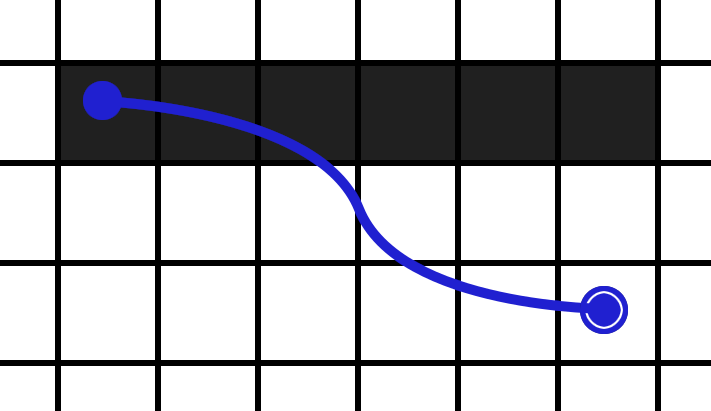
\includegraphics[width=0.25\textwidth]{images/swipe_gesture.png}
    \caption{Wizualizacja wykorzystania gestu przesunięcia}
\end{figure}


\subsection{Wykorzystanie solvera}
    Będąc na ekranie głównym można przejść do zakładki solvera poprzez naciśnięcie ikony robota.
Wyświetlona zostanie lista łamigłówek dla solvera. Początkowo, lista jest pusta, i dostępne są jedynie
predefiniowane łamigłówki dla solvera. Nową łamigłówkę można wprowadzić naciskając przycisk dodania
łamigłówki, oznaczony symbolem \textit{+}.

    Wprowadzanie opiera się na definiowaniu wskazówek, jedna po drugiej. By dodać kolejną liczbę do
wskazówki, należy nacisnąć przycisk \textit{+} na dole (z prawej dla wierszy). Jeśli wskazówka jest 
pusta (składa się jedynie z 0) to zamiast nowej liczby, aplikacja oznaczy to pole do edycji. 
Nowe wskazówki można dodać naciskająć przycisk \textit{+} z prawej (na dole dla wierszy). 
By usunąć wskazówkę, należy przytrzymać przycisk \textit{-}. Opcjonalnie można dodać tytuł dla łamigłówki.
Kreacja kończy się przyciskiem \textit{Add}.

    Przejście do łamigłówki otworzy ekran solvera. Widoczna jest na nim plansza i przycisk \textit{Solve}.
Kliknięcie przycisku rozpocznie rozwiązywanie, a po rozwiązaniu plansza zostanie zaktualizowana oraz
podany zostanie czas rozwiązania. Użytkownik może zaznaczyć dostępną opcję na ekranie, by znaleźć
wszystkie rozwiązania danej łamigłówki. Dzięki temu można przeglądać wszystkie rozwiązania danej łamigłowki
lub zweryfikować unikalność jej rozwiązania.

    By usunąć łamigłówkę, należy przytrzymać jej kartę na liście łamigłówek. Aplikacja wymaga
zatwierdzenia tej operacji.
